\documentclass[12pt,a4paper]{article}
\usepackage[utf8]{inputenc}
\usepackage[T1]{fontenc}
\usepackage{amsmath}
\usepackage{geometry}
\usepackage{setspace}
\usepackage{parskip}
\usepackage{enumitem}
\usepackage{booktabs}
\usepackage{longtable}
\usepackage{array}
\usepackage{xcolor}
\usepackage{hyperref}
\usepackage{float}
\usepackage{tikz}
\usetikzlibrary{arrows.meta,positioning,calc,matrix}
\usepackage{fancyhdr}
\usepackage{titlesec}

\geometry{left=2.5cm,right=2.5cm,top=2.5cm,bottom=2.5cm,headheight=14.5pt}
\onehalfspacing
\hypersetup{colorlinks=true,linkcolor=black,urlcolor=blue,pdftitle={Diagramas C4 - Sistema Integral de Gestión de Eventos},pdfauthor={Samuel Contreras}}

\definecolor{azul}{RGB}{31,78,121}
\definecolor{gris}{RGB}{242,242,242}
\definecolor{grisoscuro}{RGB}{80,80,80}
\definecolor{verde}{RGB}{39,120,70}
\definecolor{naranja}{RGB}{230,126,34}
\definecolor{morado}{RGB}{106,27,154}

\titleformat{\section}{\Large\bfseries\color{azul}}{\thesection.}{0.5em}{}
\titleformat{\subsection}{\large\bfseries}{\thesubsection.}{0.5em}{}
% Etiquetas en español (sin babel, que no está disponible en este entorno)
\renewcommand{\contentsname}{Índice}
\renewcommand{\figurename}{Figura}
\renewcommand{\tablename}{Tabla}

\pagestyle{fancy}
\fancyhf{}
\fancyhead[L]{Sistema Integral de Gestión de Eventos}
\fancyhead[R]{Diagramas C4}
\fancyfoot[C]{\thepage}

\begin{document}

\begin{titlepage}
\centering
\vspace*{2cm}
{\Huge\bfseries Sistema Integral de Gestión de Eventos\par}
\vspace{0.7cm}
{\Large Arquitectura de Software\par}
\vspace{1.2cm}
{\Large\bfseries Diagramas de Arquitectura --- Modelo C4\par}
\vspace{2cm}
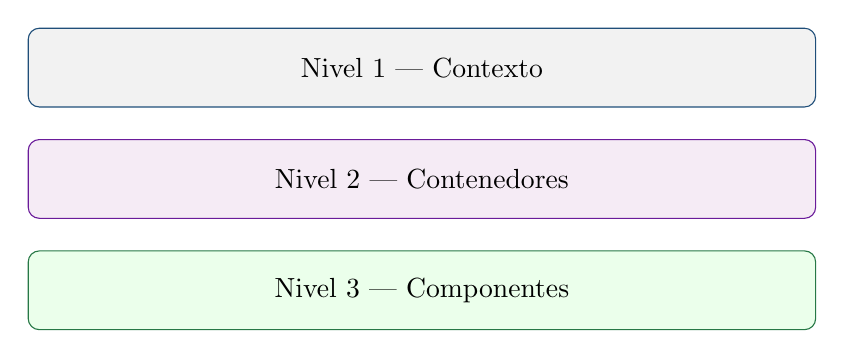
\begin{tikzpicture}
\node[draw=azul,rounded corners,fill=gris,minimum width=10cm,minimum height=1cm,align=center]
{Nivel 1 --- Contexto};
\node[draw=morado,rounded corners,fill=violet!8,minimum width=10cm,minimum height=1cm,below=0.4cm of current bounding box.south,align=center]
{Nivel 2 --- Contenedores};
\node[draw=verde,rounded corners,fill=green!8,minimum width=10cm,minimum height=1cm,below=0.4cm of current bounding box.south,align=center]
{Nivel 3 --- Componentes};
\end{tikzpicture}
\vfill
\begin{tabular}{rl}
\textbf{Materia:} & Arquitectura de Software\\
\textbf{Estudiante:} & Samuel Contreras\\
\textbf{Fecha:} & Agosto de 2026\\
\textbf{Documento base:} & Atributos de Calidad y Propuesta Arquitectónica
\end{tabular}
\end{titlepage}

\tableofcontents
\newpage

\section{Introducción}

Este documento complementa a \textbf{Atributos de Calidad y Propuesta Arquitectónica} y presenta,
de forma independiente, los diagramas de arquitectura del \textbf{Sistema Integral de Gestión de
Eventos} siguiendo el \textbf{modelo C4} (Simon Brown): \textbf{Contexto} (Nivel 1),
\textbf{Contenedores} (Nivel 2) y \textbf{Componentes} (Nivel 3). No se incluye el Nivel 4
(Código) porque la guía oficial del modelo solo lo recomienda para componentes especialmente
críticos, y normalmente se genera de forma automática con herramientas de IDE.

Cada diagrama incluye título, tipo, alcance, leyenda de notación y una tabla de relaciones con la
tecnología asociada a cada una, en cumplimiento del checklist oficial de
\href{https://c4model.com/diagrams/checklist}{c4model.com/diagrams/checklist}, verificado al
final de este documento.

\section{Nivel 1 — Diagrama de contexto}

\textbf{Tipo:} diagrama de contexto del sistema. \textbf{Alcance:} muestra el Sistema Integral de
Gestión de Eventos como caja negra, los roles de usuario que interactúan con él y los sistemas
externos de los que depende. \textbf{Audiencia:} técnica y no técnica.

\begin{figure}[H]
\centering
\resizebox{\textwidth}{!}{
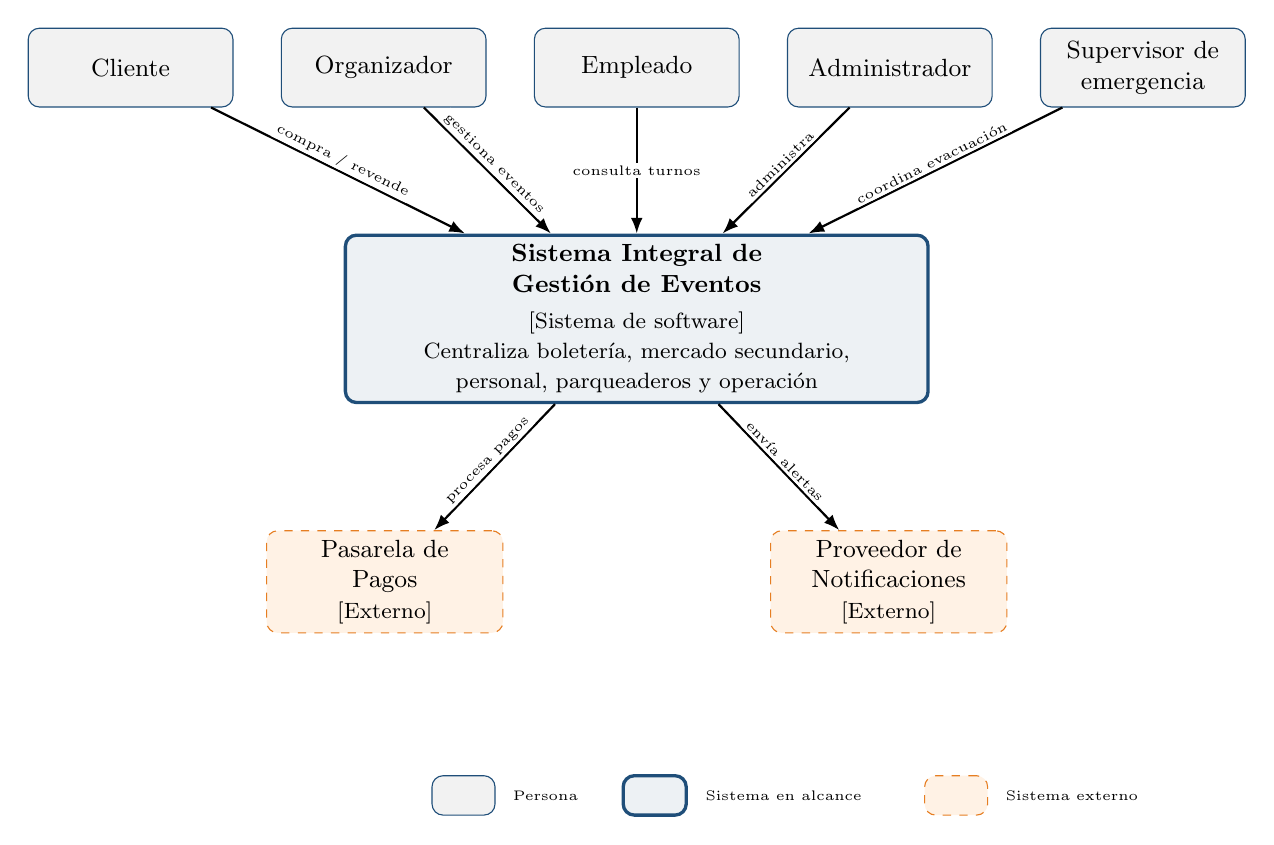
\begin{tikzpicture}[
persona/.style={draw=azul,rounded corners,fill=gris,minimum width=2.6cm,minimum height=1cm,align=center,font=\small},
sistemabox/.style={draw=azul,very thick,rounded corners,fill=azul!8,minimum width=7.4cm,minimum height=2.1cm,align=center,font=\small},
ext/.style={draw=naranja,rounded corners,dashed,fill=orange!10,minimum width=3cm,minimum height=1cm,align=center,font=\small},
arr/.style={-{Latex[length=2mm]},thick},
lbl/.style={font=\tiny,fill=white,inner sep=1pt}
]
\node[persona] (cliente) {Cliente};
\node[persona,right=6mm of cliente] (organizador) {Organizador};
\node[persona,right=6mm of organizador] (empleado) {Empleado};
\node[persona,right=6mm of empleado] (admin) {Administrador};
\node[persona,right=6mm of admin] (supervisor) {Supervisor de\\emergencia};

\node[sistemabox,below=16mm of empleado] (sistema)
  {\textbf{Sistema Integral de}\\\textbf{Gestión de Eventos}\\[2pt]
  \footnotesize [Sistema de software]\\
  \footnotesize Centraliza boletería, mercado secundario,\\
  \footnotesize personal, parqueaderos y operación};

\node[ext,below=16mm of sistema,xshift=-32mm] (pagos) {Pasarela de\\Pagos\\\footnotesize [Externo]};
\node[ext,below=16mm of sistema,xshift=32mm] (notif) {Proveedor de\\Notificaciones\\\footnotesize [Externo]};

\draw[arr] (cliente) -- (sistema) node[lbl,midway,sloped,above] {compra / revende};
\draw[arr] (organizador) -- (sistema) node[lbl,midway,sloped,above] {gestiona eventos};
\draw[arr] (empleado) -- (sistema) node[lbl,midway] {consulta turnos};
\draw[arr] (admin) -- (sistema) node[lbl,midway,sloped,above] {administra};
\draw[arr] (supervisor) -- (sistema) node[lbl,midway,sloped,above] {coordina evacuación};
\draw[arr] (sistema) -- (pagos) node[lbl,midway,sloped,above] {procesa pagos};
\draw[arr] (sistema) -- (notif) node[lbl,midway,sloped,above] {envía alertas};

\node[persona,minimum width=8mm,minimum height=5mm,font=\tiny,below=18mm of pagos,xshift=10mm] (leg1) {};
\node[font=\tiny,right=1mm of leg1] {Persona};
\node[sistemabox,minimum width=8mm,minimum height=5mm,font=\tiny,right=16mm of leg1] (leg2) {};
\node[font=\tiny,right=1mm of leg2] {Sistema en alcance};
\node[ext,minimum width=8mm,minimum height=5mm,font=\tiny,right=30mm of leg2] (leg3) {};
\node[font=\tiny,right=1mm of leg3] {Sistema externo};
\end{tikzpicture}
}
\caption{Diagrama de contexto (Nivel 1, modelo C4).}
\end{figure}

\begin{longtable}{p{3cm}p{3cm}p{6.5cm}p{2.3cm}}
\toprule
\textbf{Origen} & \textbf{Destino} & \textbf{Descripción} & \textbf{Tecnología}\\
\midrule
Cliente & Sistema & Consulta eventos, compra y revende entradas, reserva parqueadero. & HTTPS\\
Organizador & Sistema & Crea eventos, asigna personal y coordina la operación. & HTTPS\\
Empleado & Sistema & Consulta turnos y registra ingreso/salida. & HTTPS\\
Administrador & Sistema & Administra usuarios, personal y configuración. & HTTPS\\
Supervisor de emergencia & Sistema & Activa y coordina el protocolo de evacuación. & HTTPS\\
Sistema & Pasarela de Pagos & Procesa compras, reventas y reembolsos. & HTTPS/REST\\
Sistema & Proveedor de Notificaciones & Envía notificaciones push, correo y SMS. & HTTPS/REST\\
\bottomrule
\caption{Relaciones del diagrama de contexto.}
\end{longtable}

\section{Nivel 2 — Diagrama de contenedores}

\textbf{Tipo:} diagrama de contenedores. \textbf{Alcance:} zoom dentro del sistema, mostrando las
aplicaciones desplegables, los microservicios de dominio y la infraestructura de soporte.
\textbf{Audiencia:} arquitectos y desarrolladores.

\begin{figure}[H]
\centering
\resizebox{\textwidth}{!}{
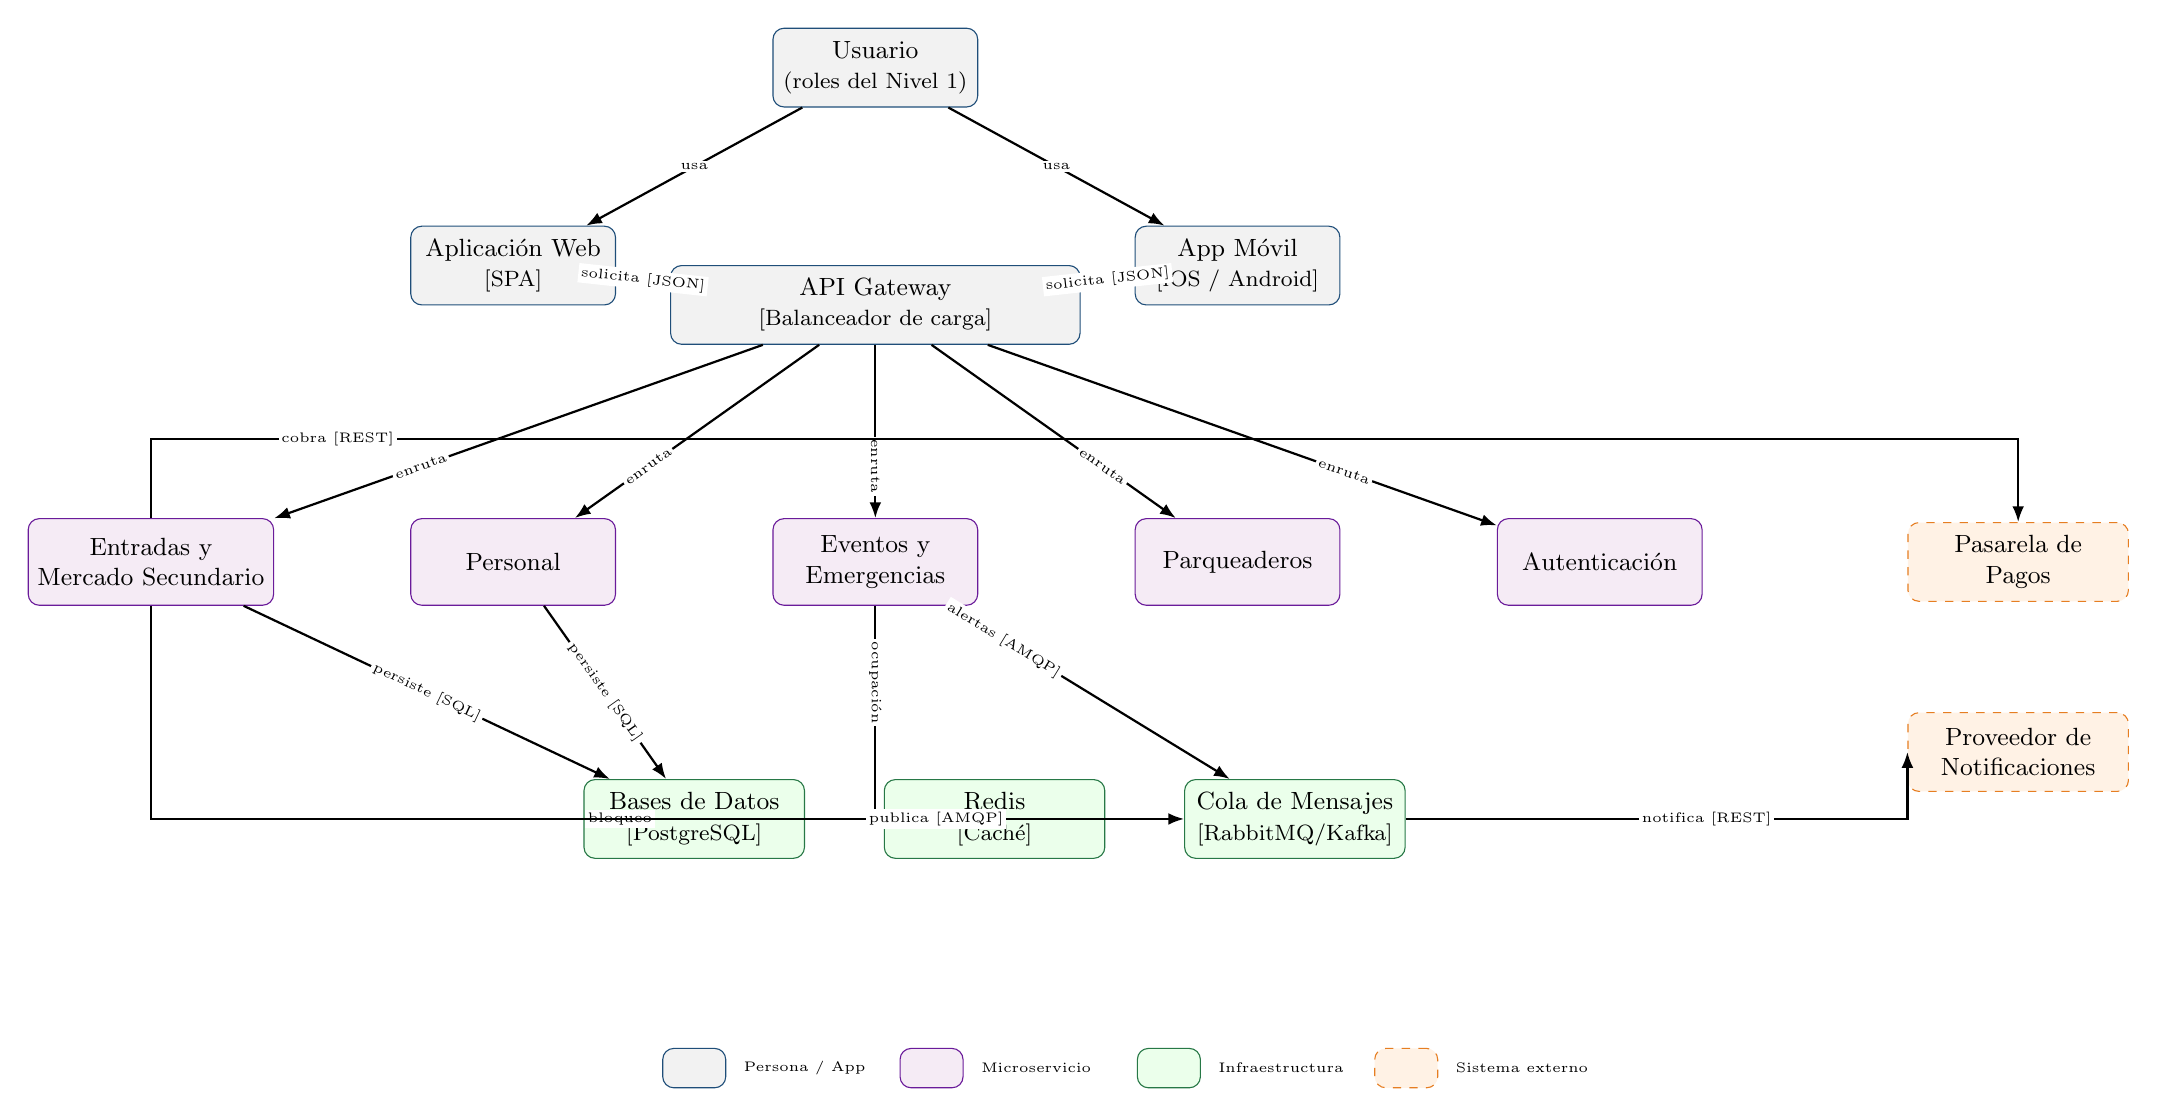
\begin{tikzpicture}[
persona/.style={draw=azul,rounded corners,fill=gris,minimum width=2.6cm,minimum height=1cm,align=center,font=\small},
contenedor/.style={draw=azul,rounded corners,fill=gris,minimum width=2.6cm,minimum height=1cm,align=center,font=\small},
microservicio/.style={draw=morado,rounded corners,fill=violet!8,minimum width=2.6cm,minimum height=1.1cm,align=center,font=\small},
infra/.style={draw=verde,rounded corners,fill=green!8,minimum width=2.8cm,minimum height=1cm,align=center,font=\small},
ext/.style={draw=naranja,rounded corners,dashed,fill=orange!10,minimum width=2.8cm,minimum height=1cm,align=center,font=\small},
arr/.style={-{Latex[length=2mm]},thick},
lbl/.style={font=\tiny,fill=white,inner sep=1pt}
]
\node[persona] (usuario) {Usuario\\\footnotesize (roles del Nivel 1)};

\node[contenedor,below=15mm of usuario,xshift=-46mm] (web) {Aplicación Web\\\footnotesize [SPA]};
\node[contenedor,below=15mm of usuario,xshift=46mm] (movil) {App Móvil\\\footnotesize [iOS / Android]};

\node[contenedor,below=20mm of usuario,minimum width=5.2cm] (gw) {API Gateway\\\footnotesize [Balanceador de carga]};

\node[microservicio,below=22mm of gw,xshift=-92mm] (ms1) {Entradas y\\Mercado Secundario};
\node[microservicio,below=22mm of gw,xshift=-46mm] (ms2) {Personal};
\node[microservicio,below=22mm of gw] (ms3) {Eventos y\\Emergencias};
\node[microservicio,below=22mm of gw,xshift=46mm] (ms4) {Parqueaderos};
\node[microservicio,below=22mm of gw,xshift=92mm] (ms5) {Autenticación};

\node[infra,below=22mm of ms2,xshift=23mm] (bd) {Bases de Datos\\\footnotesize [PostgreSQL]};
\node[infra,right=10mm of bd] (redis) {Redis\\\footnotesize [Caché]};
\node[infra,right=10mm of redis] (cola) {Cola de Mensajes\\\footnotesize [RabbitMQ/Kafka]};

\node[ext,right=26mm of ms5] (pagos2) {Pasarela de\\Pagos};
\node[ext,below=14mm of pagos2] (notif2) {Proveedor de\\Notificaciones};

\draw[arr] (usuario) -- (web) node[lbl,midway] {usa};
\draw[arr] (usuario) -- (movil) node[lbl,midway] {usa};
\draw[arr] (web) -- (gw) node[lbl,midway,sloped] {solicita [JSON]};
\draw[arr] (movil) -- (gw) node[lbl,midway,sloped] {solicita [JSON]};
\foreach \m in {ms1,ms2,ms3,ms4,ms5} \draw[arr] (gw) -- (\m) node[lbl,pos=0.7,sloped] {enruta};

\draw[arr] (ms1) -- (bd) node[lbl,midway,sloped] {persiste [SQL]};
\draw[arr] (ms2) -- (bd) node[lbl,midway,sloped] {persiste [SQL]};
\draw[arr] (ms1) |- (redis) node[lbl,pos=0.82] {bloqueo};
\draw[arr] (ms3) |- (redis) node[lbl,pos=0.18,sloped] {ocupación};
\draw[arr] (ms1) |- (cola) node[lbl,pos=0.88] {publica [AMQP]};
\draw[arr] (ms3) -- (cola) node[lbl,pos=0.2,sloped] {alertas [AMQP]};
\draw[arr] (ms1.north) |- ($(ms1.north)+(0,10mm)$) -| (pagos2.north) node[lbl,pos=0.05,sloped] {cobra [REST]};
\draw[arr] (cola.east) -| (notif2.west) node[lbl,pos=0.3] {notifica [REST]};

\node[persona,minimum width=8mm,minimum height=5mm,font=\tiny,below=24mm of bd] (leg1) {};
\node[font=\tiny,right=1mm of leg1] {Persona / App};
\node[microservicio,minimum width=8mm,minimum height=5mm,font=\tiny,right=22mm of leg1] (leg2) {};
\node[font=\tiny,right=1mm of leg2] {Microservicio};
\node[infra,minimum width=8mm,minimum height=5mm,font=\tiny,right=22mm of leg2] (leg3) {};
\node[font=\tiny,right=1mm of leg3] {Infraestructura};
\node[ext,minimum width=8mm,minimum height=5mm,font=\tiny,right=22mm of leg3] (leg4) {};
\node[font=\tiny,right=1mm of leg4] {Sistema externo};
\end{tikzpicture}
}
\caption{Diagrama de contenedores (Nivel 2, modelo C4).}
\end{figure}

\begin{longtable}{p{3.2cm}p{3.2cm}p{5.7cm}p{2.3cm}}
\toprule
\textbf{Origen} & \textbf{Destino} & \textbf{Descripción} & \textbf{Tecnología}\\
\midrule
App Web / Móvil & API Gateway & Envía las solicitudes del usuario al backend. & HTTPS/JSON\\
API Gateway & Microservicios & Enruta cada solicitud al servicio correspondiente y balancea la carga. & HTTPS/JSON\\
Servicio de Entradas & Bases de Datos & Persiste entradas, publicaciones y transferencias. & SQL\\
Servicio de Entradas & Redis & Bloquea temporalmente una publicación durante el checkout. & Redis\\
Eventos/Emergencias & Redis & Actualiza el estado de ocupación de zonas en tiempo real. & Redis\\
Servicio de Entradas & Cola de Mensajes & Publica el evento de transferencia completada. & AMQP\\
Eventos/Emergencias & Cola de Mensajes & Publica alertas de evacuación. & AMQP\\
Servicio de Entradas & Pasarela de Pagos & Procesa el cobro de una compra o reventa. & HTTPS/REST\\
Cola de Mensajes & Proveedor de Notificaciones & Dispara notificaciones push, correo y SMS. & HTTPS/REST\\
\bottomrule
\caption{Relaciones del diagrama de contenedores.}
\end{longtable}

\section{Nivel 3 — Diagrama de componentes}

\textbf{Tipo:} diagrama de componentes. \textbf{Alcance:} zoom dentro del contenedor
\textit{Servicio de Entradas y Mercado Secundario} (caso de uso complejo CU-016), mostrando sus
componentes internos y su relación con los contenedores de los niveles anteriores.
\textbf{Audiencia:} arquitectos y desarrolladores.

\begin{figure}[H]
\centering
\resizebox{\textwidth}{!}{
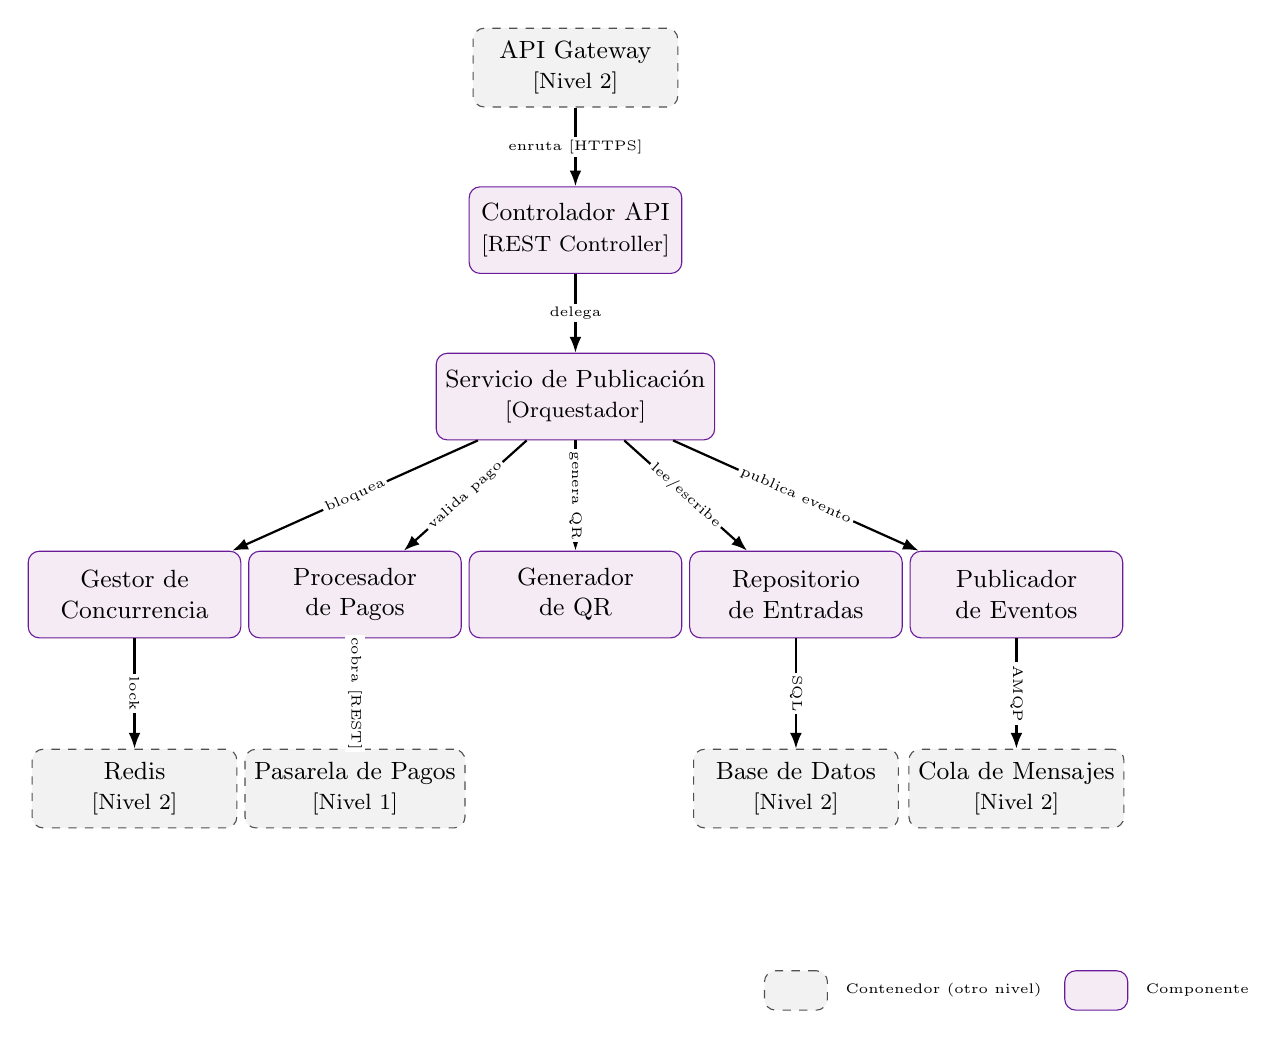
\begin{tikzpicture}[
referencia/.style={draw=grisoscuro,rounded corners,dashed,fill=gris,minimum width=2.6cm,minimum height=1cm,align=center,font=\small},
componente/.style={draw=morado,rounded corners,fill=violet!8,minimum width=2.7cm,minimum height=1.1cm,align=center,font=\small},
arr/.style={-{Latex[length=2mm]},thick},
lbl/.style={font=\tiny,fill=white,inner sep=1pt}
]
\node[referencia] (gw) {API Gateway\\\footnotesize [Nivel 2]};
\node[componente,below=10mm of gw] (ctrl) {Controlador API\\\footnotesize [REST Controller]};
\node[componente,below=10mm of ctrl] (pub) {Servicio de Publicación\\\footnotesize [Orquestador]};

\node[componente,below=14mm of pub,xshift=-56mm] (conc) {Gestor de\\Concurrencia};
\node[componente,below=14mm of pub,xshift=-28mm] (pago) {Procesador\\de Pagos};
\node[componente,below=14mm of pub] (qr) {Generador\\de QR};
\node[componente,below=14mm of pub,xshift=28mm] (repo) {Repositorio\\de Entradas};
\node[componente,below=14mm of pub,xshift=56mm] (evt) {Publicador\\de Eventos};

\node[referencia,below=14mm of conc] (redis) {Redis\\\footnotesize [Nivel 2]};
\node[referencia,below=14mm of pago] (pasarela) {Pasarela de Pagos\\\footnotesize [Nivel 1]};
\node[referencia,below=14mm of repo] (bd) {Base de Datos\\\footnotesize [Nivel 2]};
\node[referencia,below=14mm of evt] (cola) {Cola de Mensajes\\\footnotesize [Nivel 2]};

\draw[arr] (gw) -- (ctrl) node[lbl,midway] {enruta [HTTPS]};
\draw[arr] (ctrl) -- (pub) node[lbl,midway] {delega};
\draw[arr] (pub) -- (conc) node[lbl,midway,sloped] {bloquea};
\draw[arr] (pub) -- (pago) node[lbl,midway,sloped] {valida pago};
\draw[arr] (pub) -- (qr) node[lbl,midway,sloped] {genera QR};
\draw[arr] (pub) -- (repo) node[lbl,midway,sloped] {lee/escribe};
\draw[arr] (pub) -- (evt) node[lbl,midway,sloped] {publica evento};
\draw[arr] (conc) -- (redis) node[lbl,midway,sloped] {lock};
\draw[arr] (pago) -- (pasarela) node[lbl,midway,sloped] {cobra [REST]};
\draw[arr] (repo) -- (bd) node[lbl,midway,sloped] {SQL};
\draw[arr] (evt) -- (cola) node[lbl,midway,sloped] {AMQP};

\node[referencia,minimum width=8mm,minimum height=5mm,font=\tiny,below=18mm of bd] (leg1) {};
\node[font=\tiny,right=1mm of leg1] {Contenedor (otro nivel)};
\node[componente,minimum width=8mm,minimum height=5mm,font=\tiny,right=30mm of leg1] (leg2) {};
\node[font=\tiny,right=1mm of leg2] {Componente};
\end{tikzpicture}
}
\caption{Diagrama de componentes — Servicio de Entradas y Mercado Secundario (Nivel 3, modelo C4).}
\end{figure}

\begin{longtable}{p{3.2cm}p{3.2cm}p{5.7cm}p{2.3cm}}
\toprule
\textbf{Origen} & \textbf{Destino} & \textbf{Descripción} & \textbf{Tecnología}\\
\midrule
API Gateway & Controlador API & Enruta la solicitud del cliente hacia el servicio. & HTTPS/JSON\\
Controlador API & Servicio de Publicación & Delega la validación y orquestación de la reventa. & Llamada interna\\
Servicio de Publicación & Gestor de Concurrencia & Solicita el bloqueo temporal de la entrada. & Llamada interna\\
Gestor de Concurrencia & Redis & Escribe y consulta el estado del bloqueo. & Redis\\
Servicio de Publicación & Procesador de Pagos & Solicita la validación y cobro del pago. & Llamada interna\\
Procesador de Pagos & Pasarela de Pagos & Procesa el cobro de la transacción. & HTTPS/REST\\
Servicio de Publicación & Generador de QR & Invalida el QR anterior y genera uno nuevo. & Llamada interna\\
Servicio de Publicación & Repositorio de Entradas & Lee y actualiza los datos de la entrada. & Llamada interna\\
Repositorio de Entradas & Base de Datos & Consulta y persiste los registros. & SQL\\
Servicio de Publicación & Publicador de Eventos & Publica el evento de transferencia completada. & Llamada interna\\
Publicador de Eventos & Cola de Mensajes & Publica el mensaje para notificación y liquidación. & AMQP\\
\bottomrule
\caption{Relaciones del diagrama de componentes.}
\end{longtable}

\section{Verificación contra el checklist oficial de C4}

Los tres diagramas se validaron contra el
\href{https://c4model.com/diagrams/checklist}{\textit{Software architecture diagram review checklist}}
de c4model.com.

\begin{longtable}{p{9.5cm}p{2cm}}
\toprule
\textbf{Criterio (General)} & \textbf{Cumple}\\
\midrule
¿El diagrama tiene título? & Sí\\
¿Se entiende el tipo de diagrama? & Sí\\
¿Se entiende el alcance del diagrama? & Sí\\
¿El diagrama tiene leyenda/clave? & Sí\\
\midrule
\textbf{Criterio (Elementos)} & \textbf{Cumple}\\
\midrule
¿Cada elemento tiene nombre? & Sí\\
¿Se entiende el tipo de cada elemento (persona, sistema, contenedor, componente)? & Sí\\
¿Se entiende qué hace cada elemento? & Sí\\
¿Se entienden las tecnologías asociadas a cada elemento? & Sí\\
¿Se entiende el significado de los colores usados? & Sí (ver leyenda)\\
¿Se entiende el significado de los bordes punteados? & Sí (punteado = externo / referencia a otro nivel)\\
\midrule
\textbf{Criterio (Relaciones)} & \textbf{Cumple}\\
\midrule
¿Cada flecha tiene una etiqueta que describe la relación? & Sí\\
¿La descripción coincide con la dirección de la flecha? & Sí\\
¿Se entienden las tecnologías/protocolos de cada relación? & Sí (ver tablas de relaciones)\\
¿Se entiende el significado de las cabezas de flecha? & Sí (una sola convención en todo el documento)\\
\bottomrule
\caption{Verificación contra el checklist de c4model.com.}
\end{longtable}

\section{Conclusión}

Los tres niveles del modelo C4 documentan de forma progresiva la arquitectura del Sistema
Integral de Gestión de Eventos: desde su relación con los usuarios y sistemas externos (Nivel 1),
pasando por sus aplicaciones, microservicios e infraestructura de soporte (Nivel 2), hasta el
detalle interno del componente más complejo del sistema, el Servicio de Entradas y Mercado
Secundario (Nivel 3, CU-016). Cada diagrama fue verificado contra el checklist oficial de
c4model.com, garantizando que título, alcance, leyenda, tipos de elemento y tecnologías de cada
relación queden explícitos. Este documento debe leerse en conjunto con \textit{Atributos de
Calidad y Propuesta Arquitectónica}, que sustenta las decisiones que aquí se representan
gráficamente.

\end{document}
